\documentclass[12pt, a4paper, twoside]{book}
\usepackage[utf8]{inputenc} % Aceptar diferentes tipos de codificación de caracteres de entrada (en este caso usamos la codificación Unicode UTF-8)
%\usepackage{natbib}
\usepackage{listings}
\usepackage{eurosym}
\usepackage[spanish]{babel}
\usepackage{titlesec}
\usepackage{graphicx} % Soporte aumentado para gráficos 
\usepackage{float}
\usepackage{hyperref} % Para manejar referencias cruzadas. P.ej. añadir hiperenlaces al índice
\usepackage{caption}
\usepackage{setspace}
\usepackage{color}
\usepackage[a4paper, top=3.5cm, bottom=3.5cm, left=3cm, right=3cm]{geometry}
\spacing{1.5}
\setcounter{secnumdepth}{4}
\setlength{\parindent}{12pt}
\titleformat{\paragraph}
{\normalfont\normalsize\bfseries}{\theparagraph}{1em}{}
\titlespacing*{\paragraph}
{0pt}{3.25ex plus 1ex minus .2ex}{1.5ex plus .2ex}

%\usepackage{inconsolata}
%
%\usepackage[T1]{fontenc}
%
%\definecolor{pblue}{rgb}{0.13,0.13,1}
%\definecolor{pgreen}{rgb}{0,0.5,0}
%\definecolor{pred}{rgb}{0.9,0,0}
%\definecolor{pgrey}{rgb}{0.46,0.45,0.48}
%
%\lstset{language=Java,
%	showspaces=false,
%	showtabs=false,
%	breaklines=true,
%	showstringspaces=false,
%	breakatwhitespace=true,
%	commentstyle=\color{pgreen},
%	keywordstyle=\color{pblue},
%	stringstyle=\color{pred},
%	basicstyle=\ttfamily,
%	moredelim=[il][\textcolor{pgrey}]{$$},
%	moredelim=[is][\textolor{pgrey}]{\%\%}{\%%}
%}


\begin{document}	
	
	\thispagestyle{empty} 	
	%%%%%%%%%%%%%%%%%%%%%%%%%%%%%%%%%%%%%%%%%%%%%%%%%%%%%%%%%%%%%%%%%%%%%%%%%%%%%%%%
	% PORTADA
	%%%%%%%%%%%%%%%%%%%%%%%%%%%%%%%%%%%%%%%%%%%%%%%%%%%%%%%%%%%%%%%%%%%%%%%%%%%%%%%%
	
	\begin{center}		
		
\includegraphics[width=15cm]{Imagenes/Simbolo_logo_UDC.png}
	\end{center}
	
	% Lista de tamaños: \Huge, \huge, \LARGE, \Large, \large, \small, \footnotesize, \tiny
	\vspace{2cm}
	
	\begin{center}		
		{\textbf{ FACULTADE DE INFORMÁTICA}}
		
		\vspace{1cm}
		\LARGE{ TRABALLO FIN DE MÁSTER }	\\
		\LARGE{ MÁSTER UNIVERSITARIO EN INGENIERÍA INFORMÁTICA } \\
		\vspace{1cm}	
		\LARGE{\textbf{ Aplicación web para a xestión de menús domésticos con servizos nutricionais : Eat Fit Week! }}
	\end{center}
	
	\vspace{2cm}
	\hfill \textbf{Autor: \textit{Elías Ferreiro Borreiros}}
	
	
	\hfill \textbf{Director: \textit{Juan José Sánchez Penas}} 
	
	
	\hfill A Coruña, Agosto, 2019					
	
	\clearpage
	
	\begin{center}
		\LARGE{\textbf{ RESUMEN }}	
	\end{center}
	Hoy en día, con el cambio en los estilos de vida de las personas y tendiendo hacia unas costumbres más sedentarias, hay una mayor necesidad de enfocarse en una dieta equilibrada y saludable.
	Para ello, se han desarrollado muchos sistemas webs y móviles para la gestión de comidas y de sus valores nutricionales.	Sin embargo, analizando esos sistemas, vemos que tienen un error en su planteamiento al inundar a los usuarios con formularios sobrecargados y repletos de información innecesaria. 
	El otro problema principal de estos sistemas es la cantidad exagerada de trabajo manual que debe hacer el usuario antes de poder disfrutar de la funcionalidad principal. 
	
	Para resolver todo esto, hemos decidido plantear el desarrollo de una aplicación que solvente estos problemas y ofrezca una funcionalidad que no disponen los competidores : el análisis nutricional dinámico de las comidas planificadas para la semana configurable por el usuario. está sobrepasando.
	
	A mayores permitiremos la gestión de las entidades necesarias para esta planificación: ingredientes, platos, menús ... 
	Esto se hará siguiendo la filosofía inicial del proyecto: simplificar la entrada lo más posible y disminuir el esfuerzo requerido por el usuario. 
	Para esto llamaremos a servicios externos que nos permitirán estimar las características nutricionales de los ingredientes de forma que el usuario no tendrá que indicar esos datos y permitiremos con cada registro de usuario el alta automática de unos ingredientes base utilizables en la mayoría de recetas que agilizarán la configuración necesaria de un nuevo perfil para permitir disfrutar al máximo al usuario de las funcionalidades realmente importantes desde el momento más temprano posible.
	
	\clearpage
	
	\textbf{Título:} Aplicación web para a xestión de menús domésticos con servizos nutricionais
	\\
	\textbf{Autor:} Elías Ferreiro Borreiros
	\\
	\textbf{Tutor/Director:} Juan José Sánchez Penas
	
	
	\textbf{Palabras clave:} Java EE, POJO, Maven, Angular JS, Spring, Hibernate, Web, MySQL, Tarea, Lista, Contexto, Cliente - Servidor, Food, Planning, Management, Scrum. 
	
	
	\renewcommand{\contentsname}{Índice de contenidos}
	\renewcommand{\listfigurename}{Índice de figuras}
	\renewcommand{\listtablename}{Índice de tablas}
	
	\tableofcontents % indice de contenidos
	
	\listoffigures % indice de figuras
	
	\listoftables % indice de tablas
	
	\clearpage
	
	\chapter{REQUISITOS DEL SISTEMA}
	\section{Introducción}
	En esta sección analizaremos los aspectos que debe cumplimentar nuestro sistema:
	
	El objetivo de este proyecto es el desarrollar un sistema que permita al usuario planificar sus comidas semanalmente haciendo un seguimiento cercano de las características nutricionales de esas comidas y permitiendo al usuario indicar un límite en esos stats que podrá verificar que cumple con su planificación semanal.
	A mayores, se llevará una gestión de ingredientes y platos registrados y mantenidos por el usuario. Con los platos que da de alta el usuario se podrán montar menús semanales sobre los que hacer seguimiento.
	Estos menús deben permitir generarse automáticamente o bien de forma aleatoria o bien de forma válida sin violar los límites indicados por el usuario. A partir del menú debemos poder obtener su lista de la compra para saber que ingredientes comprar para poder cocinarlo a lo largo de la semana, en esta lista deberíamos tener una estimación del precio que correspondería a su compra completa.
	Tendremos también una gestión de plantillas de menú para facilitar la generación de nuevos menús a través de menús previos guardados como plantillas que hayan sido de gusto para el usuario.
	
	Como requisitos técnicos no funcionales debemos hacer énfasis sobre la sencillez del diseño de los formularios para evitar inundar al usuario con gran cantidad de campos a cubrir en el alta de nuevos ingredientes y / o platos y deberíamos permitir un buen diseño visual en diferentes tamaños de pantalla al no disponer de una aplicación nativa móvil como forma de facilitar la usabilidad del usuario desde cualquier plataforma que tenga disponible.
	\section{Actores}
	\begin{itemize}
		\item Usuario: Representa la persona que utiliza nuestro sistema para recibir valor de sus funcionalidades.
		\item Sistema Estimador Nutricional (SEN): Representa al sistema externo que, al recibir la orden de nuestro sistema, estimará los valores nutricionales de un ingrediente a partir de su nombre.
		\item Sistema Scrapeador de Supermercado (SSS): Representa al sistema externo que, al recibir la orden de nuestro sistema, consultará la página de un supermercado para obtener su catálogo y sus precios.
	\end{itemize}
	\section{Casos de Uso}
	\subsection{Casos de uso Usuario}
	\subsubsection{CU-001-Registro}
	Proceso de creación de la cuenta del usuario en la aplicación. Se solicitará el email, el nombre, los apellidos y la contraseña.
	Se comprobará que el usuario introducido no existiera previamente en la aplicación y que los datos introducidos sean correctos.\\
	Precondiciones: El usuario no está registrado en la aplicación.\\
	Postcondiciones: El usuario queda registrado en la aplicación y podrá acceder a la misma.
	\subsubsection{CU-002-Login}
	Proceso de acceso a la aplicación. Se solicitarán el usuario y la contraseña y se comprobará que sean correctos. Se permitirá al usuario acceder con los datos de su cuenta de facebook.\\ 	
	Precondiciones: El usuario no está autenticado en la aplicación.\\
	Postcondiciones: No aplica.
	\subsubsection{CU-003-Logout}
	Proceso de salida de la aplicación. Solo se podrá acceder a este caso de uso estando previamente identificado en la aplicación correctamente y tras ejecutarlo, el usuario quedará desautenticado pudiendo volver a acceder con sus credenciales en cualquier momento.\\
	Precondiciones: El usuario está autenticado en la aplicación.\\
	Postcondiciones: No aplica.
	\subsubsection{CU-004-Visualizar ingredientes}
	Proceso de obtención de información de los ingredientes registrados de un usuario concreto. La información que se mostrará sobre los ingredientes será: nombre, categoría alimenticia, stats nutricionales (Calorías, Proteínas, Grasas, Carbohidratos) y se indicará una señal de advertencia en caso de que la categoría del alimento esté prohibida por el usuario.
	Para cada ingrediente se permitirá acceder a CU-005-Actualizar ingrediente y CU-007-Borrar ingrediente.\\
	Precondiciones: El usuario está autenticado en la aplicación.\\
	Postcondiciones: No aplica.
	\subsubsection{CU-005-Actualizar ingrediente}
	Proceso de actualización de la información de un ingrediente concreto registrado por el usuario.
	Se solicita al usuario la siguiente información: nombre, categoría alimenticia y stats nutricionales (Calorías, Proteínas, Grasas, Carbohidratos).
	Los campos se inicializarán con los datos del ingrediente a actualizar.
	Una vez confirmados los datos deseados y comprobado que sean correctos, la información del ingrediente correspondiente será actualizada.\\ 
	Se podrá utilizar el caso de uso SEN CU-024-Estimar ingrediente para obtener los stats nutricionales a actualizar.\\
	Precondiciones: El usuario está autenticado en la aplicación y el ingrediente a actualizar está registrado en los ingredientes del usuario.\\
	Postcondiciones: El plato queda actualizado con los nuevos datos proporcionados por el usuario.
	\subsubsection{CU-006-Añadir ingrediente}
	Proceso de creación de un nuevo ingrediente para un usuario concreto.
	Se solicita al usuario la siguiente información: nombre, categoría alimenticia y stats nutricionales (Calorías, Proteínas, Grasas, Carbohidratos).
	Una vez confirmados los datos deseados y comprobado que sean correctos, se registrará el nuevo ingrediente del usuario.\\ 
	Se podrá utilizar el caso de uso CU-000-Estimar ingrediente para obtener los stats nutricionales a actualizar.\\
	Precondiciones: El usuario está autenticado en la aplicación.\\
	Postcondiciones: No aplica.
	\subsubsection{CU-007-Borrar ingrediente}
	Proceso de borrado de un ingrediente para un usuario concreto.\\
	Precondiciones: El usuario está autenticado en la aplicación y el ingrediente a borrar está registrado en los ingredientes del usuario.\\
	Postcondiciones: El ingrediente queda borrado del sistema.
	\subsubsection{CU-008-Visualizar platos}
	Proceso de obtención de información de los platos registrados de un usuario concreto. La información que se mostrará sobre los platos será: nombre y stats nutricionales (Calorías, Proteínas, Grasas, Carbohidratos).
	Para cada plato se permitirá acceder a CU-009-Actualizar plato, CU-011-Borrar plato y CU-012-Añadir plato a primer hueco válido de menú.\\
	Precondiciones: El usuario está autenticado en la aplicación.\\
	Postcondiciones: No aplica.
	\subsubsection{CU-009-Actualizar plato}
	Proceso de actualización de la información de un plato concreto registrado por el usuario.
	Se solicita al usuario la siguiente información: nombre, receta, ingredientes que componen el plato (el nombre y la cantidad de cada uno de ellos).
	Los campos se inicializarán con los datos del plato a actualizar.
	Se podrán visualizar los stats nutricionales del plato para poder ver los efectos de los cambios en la composición del plato antes de confirmarlos.
	Una vez confirmados los datos deseados y comprobado que sean correctos, la información del plato correspondiente será actualizada.\\ 
	Precondiciones: El usuario está autenticado en la aplicación y el plato a actualizar está registrado en los platos del usuario.\\
	Postcondiciones: El ingrediente queda actualizado con los nuevos datos proporcionados por el usuario.
	\subsubsection{CU-010-Añadir plato}
	Proceso de registro de un nuevo plato registrado por el usuario.
	Se solicita al usuario la siguiente información: nombre, receta, ingredientes que componen el plato (el nombre y la cantidad de cada uno de ellos).
	Se podrán visualizar los stats nutricionales del plato para poder ver los efectos de los cambios en la composición del plato antes de confirmarlos.
	Una vez confirmados los datos deseados y comprobado que sean correctos, se registrará el nuevo plato con los datos informados.\\ 
	Precondiciones: El usuario está autenticado en la aplicación.\\
	Postcondiciones: El ingrediente queda registrado en los platos del usuario.
	\subsubsection{CU-011-Borrar plato}
	Proceso de borrado de un plato para un usuario concreto.\\
	Precondiciones: El usuario está autenticado en la aplicación y el plato a borrar está registrado en los platos del usuario.\\
	Postcondiciones: El plato queda borrado del sistema.
	\subsubsection{CU-012-Añadir plato a primer hueco válido de menú}
	Proceso de planificación de un plato en el menú actual del usuario en el primer hueco disponible.
	Se consulta el menú actual del usuario: Menú correspondiente con la semana en la que se encuentra el usuario al iniciar el caso de uso.
	1. En caso de que el plato tenga comidas permitidas:
	1.1 En caso de encontrarse la primera combinación ``Día de la semana - Comida permitida por el plato'' que no tenga ningún plato asignado en el menú actual
	1.1.1 Se añade el plato a esa primera combinación obtenida
	1.2 En caso de que el plato no tenga comidas permitidas, no se realiza ninguna acción
	1.1.2 En caso de no encontrarse una combinación disponible, no se realiza ninguna acción\\
	Precondiciones: El usuario está autenticado en la aplicación, tiene un menú en la semana actual y el plato a añadir está registrado en los platos del usuario.\\
	Postcondiciones: No hay.
	\subsubsection{CU-013-Visualización semanal de menús}
	Proceso de visualización del menú de la semana actual y de semanas anteriores y posteriores.
	Se selecciona inicialmente la semana en la que el usuario está usando el sistema.
	Se muestra al usuario el menú correspondiente a la semana seleccionada o se permite acceder al caso de uso CU-014-Crear menú en caso de no haber menú en la semana seleccionada.
	Se visualizan los stats nutricionales del menú actual pudiendo hacerlo de forma total para toda la semana o de forma diaria para el día de la semana seleccionado.
	Se permite cambiar la semana seleccionada por la semana siguiente o la anterior.\\
	Precondiciones: El usuario está autenticado en la aplicación.\\
	Postcondiciones: No hay.
	\subsubsection{CU-014-Crear menú}
	Proceso de creación de un nuevo menú para el usuario en la semana seleccionada.\\
	Precondiciones: El usuario está autenticado en la aplicación y no tiene menú en la semana seleccionada.\\
	Postcondiciones: El usuario dispone de un nuevo menú registrado en la semana seleccionada.
	\subsubsection{CU-015-Añadir plato a menú}
	Proceso de añadir plato a menú en un día y comida concretos.
	Se selecciona una combinación ``Día de la semana - Comida permitida por el plato'' que no tenga ningún plato asignado en el menú actual.
	Se selecciona un plato del usuario para añadir a la combinación.
	Se registra la relación menú - plato en la combinación seleccionada.\\
	Precondiciones: El usuario está autenticado en la aplicación.\\
	Postcondiciones: La relación menú - plato queda correctamente registrada.
	\subsubsection{CU-016-Sugerir plato en menú}
	Proceso de añadir plato sugerido automáticamente a menú en un día y comida concretos.
	Se selecciona una combinación ``Día de la semana - Comida permitida por el plato'' que no tenga ningún plato asignado en el menú actual.
	Se obtiene el plato más correcto para la combinación seleccionada: se predice de forma automática el plato más correcto a través de la información de todos los platos registrados en menús del usuario en función de los días en los que están registrados y las comidas en las que están registrados.
	Se registra la relación menú - plato en la combinación seleccionada.\\
	Precondiciones: El usuario está autenticado en la aplicación.\\
	Postcondiciones: La relación menú - plato queda correctamente registrada.
	\subsubsection{CU-017-Lista de la compra}
	Proceso de obtención de la lista de la compra necesaria para un menú concreto del usuario.
	Se obtiene del menú el número de veces que aparecen los ingredientes de los platos del menú y la cantidad en la que aparecen.
	Se obtiene la estimación del precio de todos los ingredientes del caso de uso SSS CU-025-Estimar precio lista de la compra
	Se muestra al usuario la información obtenida: Para cada ingrediente: su nombre, el número de veces que aparece en platos y la cantidad total de ese ingrediente entre esos platos. A mayores se muestra la estimación del precio de esa lista.\\
	Precondiciones: El usuario está autenticado en la aplicación.\\
	Postcondiciones: No hay.
	\subsubsection{CU-018-Limpiar menú}
	Proceso de borrado de los platos de un menú.
	Precondiciones: El usuario está autenticado en la aplicación y el menú a limpiar está entre los menús del usuario.\\
	Postcondiciones: Se eliminan todas las relaciones del menú con sus platos.
	\subsubsection{CU-019-Obtener menú aleatorio}
	Proceso de generación de un menú aleatorio.
	Para cada combinación ``Día de la semana - Comida'' del menú se obtiene la lista de los platos del usuario que permiten esa Comida y se selecciona un plato de ellos aleatoriamente.
	Se registra la relación menú - plato en la combinación.\\
	Precondiciones: El usuario está autenticado en la aplicación y el menú a generar aleatoriamente está entre los menús del usuario.\\
	Postcondiciones: El menú tiene todos sus huecos cubiertos con platos aleatorios válidos.
	\subsubsection{CU-020-Obtener menú válido}
	Proceso de generación de un menú válido para el usuario.
	Para cada combinación ``Día de la semana - Comida'' del menú se obtiene la lista de los platos del usuario que permiten esa Comida y se selecciona un plato de ellos que no hace que el menú incumpla las limitaciones nutricionales del usuario(Calorias maximas semanales, Proteinas maximas semanales ...). En la selección se priorizan platos que no estén ya registrados en el menú.
	Se registra la relación menú - plato en la combinación.\\
	Precondiciones: El usuario está autenticado en la aplicación y el menú a generar aleatoriamente está entre los menús del usuario.\\
	Postcondiciones: El menú tiene los máximos huecos posibles cubiertos con platos que no incumplen las limitaciones del usuario.
	\subsubsection{CU-021-Guardar menú como plantilla}
	Proceso de generación de una nueva plantilla de menú a partir de un menú del usuario.
	Se solicita al usuario un nombre para la plantilla de menú.
	Al confirmar el nombre, se registra la nueva plantilla.\\
	Precondiciones: El usuario está autenticado en la aplicación y el menú a guardar como plantillas está entre los menús del usuario.\\
	Postcondiciones: La nueva plantilla está registrada correctamente.
	\subsubsection{CU-022-Rellenar menú desde plantilla}
	Proceso de rellenado de un menú a partir de una plantilla.
	Se indica al usuario que seleccione una plantilla de entre sus plantillas registradas.
	Se registran las relaciones menú - plato correspondientes a la plantilla en el menú seleccionado.\\
	Precondiciones: El usuario está autenticado en la aplicación y el menú a rellenar desde plantilla está entre los menús del usuario.\\
	Postcondiciones: El menú tiene las relaciones con los platos registrados en la plantilla.
	\subsubsection{CU-023-Actualizar configuraciones de usuario}
	Proceso de actualización de las configuraciones del usuario para personalizar el funcionamiento del sistema.
	Se solicitan al usuario valores para sus configuraciones: Calorías máximas por semana, Proteinas máximas por semana, Grasas máximas por semana, Carbohidratos máximos por semana, Categorías alimenticias prohibidas, Comidas semanales.
	Se inicializan esos campos con los valores actuales de las configuraciones del usuario.
	Una vez confirmados los valores, se actualizan las configuraciones con estos nuevos valores.\\
	Precondiciones: El usuario está autenticado en la aplicación.\\
	Postcondiciones: Las configuraciones del usuario quedan actualizadas con los nuevos valores indicados.
	\subsection{Casos de uso Sistema Estimador Nutricional - SEN}
	\subsubsection{CU-024-Estimar ingrediente}
	Proceso de estimación de los stats nutricionales de un ingrediente a través de su nombre.
	Se consulta al sistema externo los stats nutricionales de ese ingrediente por su nombre.
	Se transforma la información obtenida para poder ser utilizada por nuestro sistema.\\
	Precondiciones: No hay.\\
	Postcondiciones: No hay.
	\subsection{Casos de uso Sistema Scrapeador de Supermercado - SSS}
	\subsubsection{CU-025-Estimar precio lista de la compra}
	Proceso de estimación del precio de una lista de la compra para su compra en un supermercado concreto.
	Se llama al servicio externo para obtener el catálogo de la página web del supermercado concreto.
	A través de ese catálogo se busca el precio de los ingredientes de la lista de la compra a estimar.
	Se suman todos esos precios y se devuelven.\\
	Precondiciones: No hay.\\
	Postcondiciones: No hay.
	\section{Modelo de Casos de uso}
	A continuación se muestra el diagrama de casos de uso global del sistema
	Este diagrama nos sirve para especificar la comunicación y comportamiento de nuestro sistema con sus sistemas externos a través de la interacción con los usuarios.
	\begin{figure}[H]
		\centering
		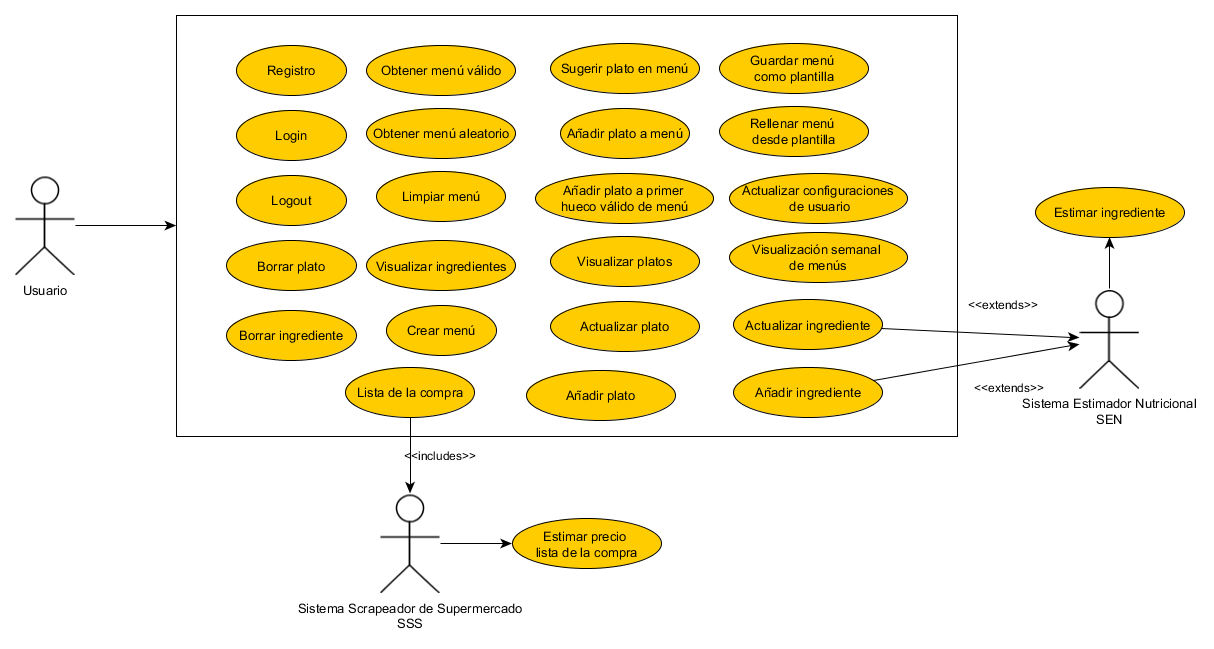
\includegraphics[width=15cm]{Imagenes/CasosUso.png}
		\caption{Casos de uso}\label{Casos de uso}
	\end{figure} 
	
\end{document}

